\documentclass[tikz,border=6pt]{standalone}
% Shared figure style for the Space Data Network whitepapers.
\usepackage{lmodern}
\usepackage[T1]{fontenc}
\usepackage{xcolor}
\usetikzlibrary{arrows.meta,positioning,calc,fit,backgrounds,matrix}
\hyphenpenalty=10000\exhyphenpenalty=10000
\definecolor{ink}{HTML}{1F2328}
\definecolor{rule}{HTML}{57606A}
\definecolor{panel}{HTML}{F3F4F6}
\definecolor{accent}{HTML}{D4880F}
\tikzset{
  every picture/.style={line width=0.6pt, draw=ink, text=ink, font=\small},
  box/.style={draw=ink, fill=panel, rounded corners=2pt, align=center, inner sep=5pt},
  plain/.style={draw=ink, fill=white, rounded corners=2pt, align=center, inner sep=5pt},
  title/.style={font=\bfseries\small},
  where/.style={font=\scriptsize\itshape, text=rule},
  note/.style={font=\footnotesize\itshape, text=rule},
  flow/.style={-{Stealth[length=2.2mm]}, draw=rule},
}

\begin{document}
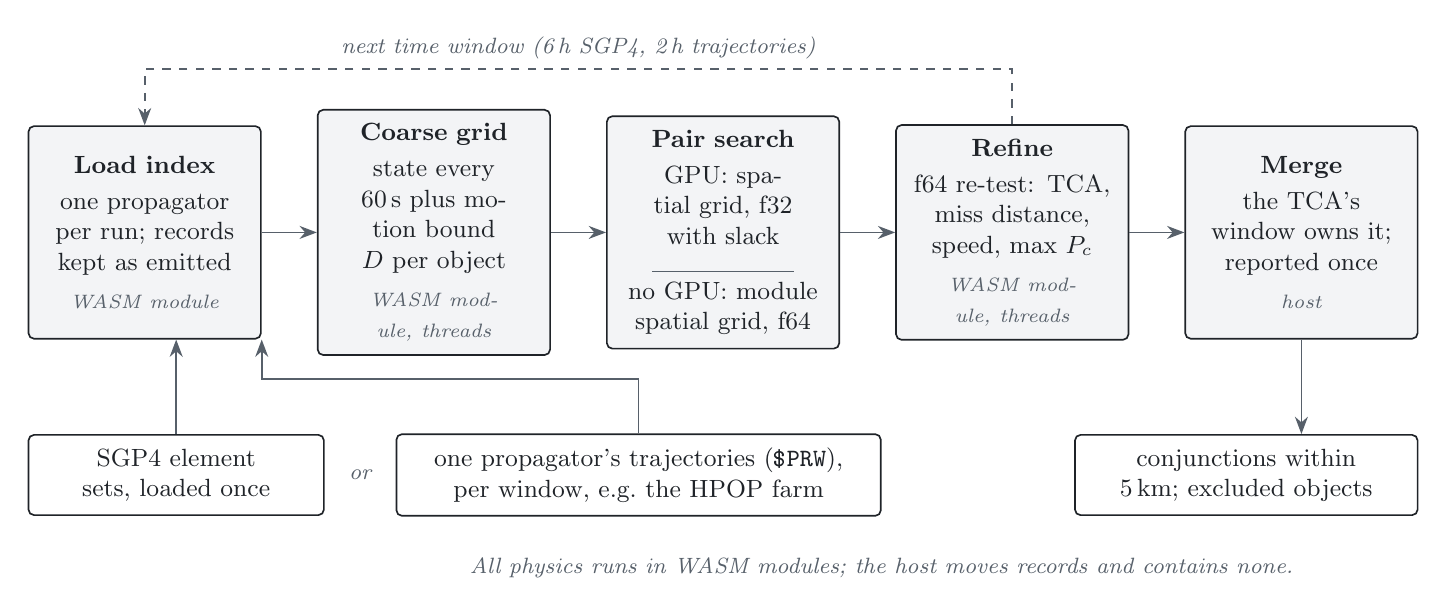
\begin{tikzpicture}[node distance=7mm, stage/.style={box, text width=26mm, minimum height=27mm}]
\node[stage] (load) {{\bfseries Load index}\\[2pt] one propagator per run; records kept as emitted\\[3pt] \textcolor{rule}{\scriptsize\itshape WASM module}};
\node[stage, right=of load] (grid) {{\bfseries Coarse grid}\\[2pt] state every 60\,s plus motion bound $D$ per object\\[3pt] \textcolor{rule}{\scriptsize\itshape WASM module, threads}};
\node[stage, right=of grid] (pair) {{\bfseries Pair search}\\[2pt] GPU: spatial grid, f32 with slack\\[-1pt] \textcolor{rule}{\rule{18mm}{0.3pt}}\\[-1pt] no GPU: module spatial grid, f64};
\node[stage, right=of pair] (refine) {{\bfseries Refine}\\[2pt] f64 re-test: TCA, miss distance, speed, max $P_c$\\[3pt] \textcolor{rule}{\scriptsize\itshape WASM module, threads}};
\node[stage, right=of refine] (merge) {{\bfseries Merge}\\[2pt] the TCA's window owns it; reported once\\[3pt] \textcolor{rule}{\scriptsize\itshape host}};
\foreach \a/\b in {load/grid, grid/pair, pair/refine, refine/merge} \draw[flow] (\a) -- (\b);
\draw[flow, dashed] (refine.north) -- ++(0,7mm) -| node[pos=0.25, above, note] {next time window (6\,h SGP4, 2\,h trajectories)} (load.north);
\node[plain, below=12mm of load.south west, anchor=north west, text width=34mm] (sgp4) {SGP4 element sets, loaded once};
\node[plain, right=9mm of sgp4, text width=58mm] (traj) {one propagator's trajectories (\texttt{\$PRW}), per window, e.g.\ the HPOP farm};
\path (sgp4) -- node[note] {or} (traj);
\node[plain, below=12mm of merge.south east, anchor=north east, text width=40mm] (out) {conjunctions within 5\,km; excluded objects};
\draw[flow] (sgp4.north) -- (sgp4.north |- load.south);
\draw[flow] (traj.north) |- ($(load.south east)+(0,-5mm)$) -- ++(0,5mm);
\draw[flow] (merge.south) -- (merge.south |- out.north);
\node[note, below=4mm of traj.south east, anchor=north] {All physics runs in WASM modules; the host moves records and contains none.};
\end{tikzpicture}
\end{document}
